\documentclass[12pt]{article}

%\usepackage{sectsty}
\usepackage{titlesec}
\usepackage{url}

\usepackage{amssymb}

\usepackage{titlesec}

\usepackage{transparent}

\usepackage{setspace}
%\doublespacing
%\onehalfspacing

\usepackage{graphicx}
%\graphicspath{ {/ext_root/openshift-oc3/mmui-caf-local/web/mmui/public/pics/} }

\newcommand{\sectionGraphics}{

\vspace{2em}\centerline{\includegraphics[scale=0.125]{logo-deco.png}}\vspace{-1em}}

\usepackage[flushmargin]{footmisc}

\setlength{\parindent}{30pt}

%\usepackage{bigfoot}

%\DeclareNewFootnote[para]{R}[Roman]
%\DeclareNewFootnote[para]{N}

%\usepackage[letterpaper, left=1.3in,right=1in,top=1in,bottom=1in]{geometry}

\newcommand{\descItem}[1]{\item[{\color{logoRed!80!logoBlue}{\fontfamily{phv}%
\fontshape{it}\fontseries{b}\selectfont\scriptsize #1}}]}
%\newcommand{\descItem}[1]{\item[#1]}

\newcommand{\descItemLarge}[1]{\item[{\color{logoRed!80!logoBlue}{\fontfamily{phv}%
\fontshape{it}\fontseries{b}\selectfont\small #1}}]}


\usepackage{enumitem}

\setlist[description]{%
  topsep=30pt,               % space before start / after end of list
  itemsep=5pt,               % space between items
  font={\bfseries\sffamily}, % set the label font
%  font={\bfseries\sffamily\color{red}}, % if colour is needed
}


\usepackage{etoolbox}

\usepackage{mathptmx}
%\usepackage{euler}
%\usepackage{amsmath}

%\usepackage[LGRgreek]{mathastext}

%\sectionfont{\fontsize{12}{15}\selectfont}
%\subsectionfont{\fontsize{11}{12}\selectfont}

\titleformat*{\subsection}{\small\bfseries}

\usepackage{eufrak}
\usepackage{wasysym}
\usepackage{textcomp}
\usepackage{amssymb}

\usepackage{microtype}


\usepackage{graphicx}

\usepackage{tikz}

\usetikzlibrary{decorations.pathmorphing}
\usetikzlibrary{positioning}
\usetikzlibrary{shapes,snakes}


\let\OldSection\section

\renewcommand\section[1]{
	\vspace{9pt}
	
	\scalebox{1.3}{\colorbox{logoPurple!50}{\hspace{1em}}}
				
	%\hspace{-1.1cm}{\protect\includegraphics[width=1cm]{e-logo.png}}	
	{\protect\transparent{0.3}{\colorbox{logoPeach!10!blue}{%
			\begin{minipage}{\linewidth}
				    \vspace{.5em}
				
	\protect\transparent{1}{\OldSection{#1%
		%{\transparent{0.5}{
		%	\protect\includegraphics[width=1cm]{e-logo.png}
		%}
	    %}
     }}
	    \end{minipage}}} }
    
    \vspace{-5em}
    	{\protect\transparent{0.3}{\colorbox{logoPeach}{%
    		\begin{minipage}{\linewidth}
    			\hspace{\linewidth}
    	\end{minipage}}} } 
    
    \vspace{5em}
    
	\vspace{-6pt}
}

%\subsectionfont{\Large}
%\subsectionfont{\fontsize{12}{15}\selectfont}

\titleformat*{\subsection}{\Large\bfseries}

\let\OldSubsection\subsection
\renewcommand\subsection[1]{

	\vspace{12pt}
	
    %{\LARGE
	%\colorbox{logoCyan}{%
	%\begin{minipage}{\linewidth}
		\OldSubsection{% 	
			\hspace{-2.75em}
			%\begin{minipage}{}
			\protect\raisebox{-5pt}{%
			\colorbox{logoCyan!50}{\hspace{2.1em}}}%
			\hspace{-5pt}{\protect\transparent{0.3}{\colorbox{logoBlue!80}{\protect\transparent{1}{%
						   \protect\raisebox{1pt}{\textit{{\large #1}}} }}}}
			%\end{minipage}
		}
	%\end{minipage}
    %}
    %}
	\vspace{-6pt}
}



\newcommand*{\MyCircle}{\begin{tikzpicture}{baseline}
	\node [draw, shape=regular polygon, regular polygon sides = 5, shape border rotate=180,
	line width=.2mm, left color=blGreen, right color=darkBlGreen, draw=darkRed, aspect=1,
	draw opacity=0.6, fill opacity=0.8, xscale=0.5, yscale=0.5,
	minimum width=1mm, 
	] 
	at (0, 0) {};
	\end{tikzpicture}}


\newcommand*{\MyLabel}{%
 %\MyBall	
 %{\tikz \draw [baseline, ball color=red, draw=red] circle (3pt);} 	
 \protect\MyCircle{\hspace{4pt}}\color{flColor}\LARGE{\textbf{\protect\raisebox{-3pt}{\theenumi}}}
}

%
\newenvironment{colorDescription}{%
\vspace{1em}\begin{description}[style=nextline]}{\end{description}}

\newcommand*{\MyDiamond}{%
	\begin{tikzpicture}{baseline}
	
	\node [draw, shape=diamond, %shape border rotate=100,
	line width=.2mm, left color=flColor, right color=darkRed, draw=logoPurple, aspect=1,
	draw opacity=0.6, fill opacity=0.8, xscale=0.5, yscale=0.5,
	minimum width=1mm, 
	] 
	at (2, 0) {};
	
	\end{tikzpicture}
	
} 

\usepackage{enumitem}

\newcommand*{\MyDiamon}{*} 


\newenvironment{colorItemize}{\vspace{1em}\begin{itemize}[label={\MyDiamond}]}{\end{itemize}}

\newenvironment{colorEnumerate}{\vspace{1em}\begin{enumerate}[label=\MyLabel]}{\end{enumerate}}

\newcommand{\PeoplesVoiceCafe}{{\relscale{0.8}{\fontfamily{fvs}\fontseries{b}\selectfont%
 Peoples' Voice Cafe}}}
 
\newcommand{\q}[1]{{\fontfamily{qcr}\selectfont ``}#1{\fontfamily{qcr}\selectfont ''}} 

\usepackage{tcolorbox}

%\usepackage[framemethod=TikZ]{mdframed}

%
\tcbuselibrary{skins}
%\tcbuselibrary{listings,breakable}
\usetikzlibrary{calc}
\usetikzlibrary{shadows}
\pgfdeclarelayer{background}
\pgfdeclarelayer{foreground}
\pgfsetlayers{background,main,foreground}

\definecolor{BaseColor}{HTML}{8533FF}

\newlength{\boxShadowOfset}
\setlength{\boxShadowOfset}{2mm}

\newcommand{\tc}[1]{
\vspace*{-2.05cm}\hspace{1cm}
\begin{tcolorbox}
[colframe=cyan!10!black,boxrule=0.5pt,arc=8pt,hbox,enhanced, 
leftrule=5pt,rightrule=3pt,toprule=0pt,toprule=0pt,
%drop fuzzy shadow southeast={BaseColor!50!white},
%frame code={
%        },
     % left=6pt,right=6pt,top=6pt,bottom=6pt,
      boxsep=0pt]      
\protect{#1}
\end{tcolorbox}      
\vspace*{0.4cm}

}

\newcommand{\cursive}[2]{{\LARGE%
%\begin{minipage}{0.5\textwidth}
\protect\tc{%
%\protect\fcolorbox{cyan!10!black}{white}{
\protect\raisebox{-2pt}{
{\color{logoBlue!90!cyan}{%
{\fontfamily{bch}\fontseries{b}\selectfont%
 \larger{#1}}}}}{{\color{logoBlue!90!cyan}{\Fontlukas\bfseries\textsc{#2}}}}%
%\end{minipage}
%}
}}}
%\end{minipage}

\newcommand{\parlead}[1]{\vspace{1.15em}\noindent{%
{\color{logoRed!80!logoBlue}{\fontfamily{bch}\fontseries{b}\selectfont\large #1}}}}

\newcommand{\itemLarger}[1]{\item {\raisebox{-2pt}{\larger{#1}}}}

\newcommand{\itemLargerLine}[2]{\item {\raisebox{-2pt}{\larger{#1}}}%
\hspace{1em}{\raisebox{-2pt}{#2}}}

\newcommand{\p}{

\vspace{.45em}}

\newcommand{\txtbl}{\hspace{2pt}{{\raisebox{1pt}{\relsize{-2}\textbullet}}}\hspace{2pt}}

\newcommand{\colorhref}[1]{\colorbox{blGreen!20}{#1}}



\PassOptionsToPackage{svgnames}{xcolor}

\usepackage[object=vectorian]{pgfornament} %%  http://altermundus.com/pages/tkz/ornament/index.html
\usepackage{lipsum,tikz}

\newcommand{\sectionline}[1]{%
  \noindent
  \begin{center}
  {\color{#1}
    \resizebox{0.5\linewidth}{1ex}
    {{%
    {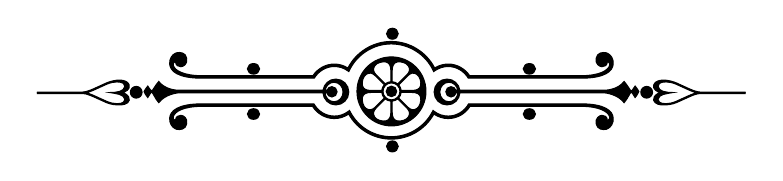
\begin{tikzpicture}
    \node  (C) at (0,0) {};
    \node (D) at (9,0) {};
    \path (C) to [ornament=84] (D);
    \end{tikzpicture}}}}}%
    \end{center}
  }
%% A macro with two arguments to change ornaments and colors easily
%% Syntax -- \sectionlinetwo{<color>}{<ornament>}
\newcommand{\sectionlinetwo}[2]{%
  \nointerlineskip \vspace{.5\baselineskip}\hspace{\fill}
  {\color{#1}
    \resizebox{0.5\linewidth}{2ex}
    {{%
    {\begin{tikzpicture}
    \node  (C) at (0,0) {};
    \node (D) at (9,0) {};
    \path (C) to [ornament=#2] (D);
    \end{tikzpicture}}}}}%
    \hspace{\fill}
    \par\nointerlineskip \vspace{.5\baselineskip}
  }

\newcommand{\EnglischeLinie}{
\sectionline{darkRed!60!cyan}
}

\newcommand{\lMOSAIC}{\mbox{MOSAIC}}
\newcommand{\lfMOSAIC}{\mbox{M\small{OSAIC}}}
\newcommand{\MOSAIC}{\mbox{\small{MOSAIC}}}
\newcommand{\RAK}{\mbox{\small{RAK}}}
\newcommand{\SDK}{\mbox{\small{SDK}}}
\newcommand{\lSDK}{\mbox{SDK}}
\newcommand{\GUI}{\mbox{\small{GUI}}}
\newcommand{\qvspace}{\vspace{.4em}}
\begin{document}\rztitle{Cognitive State Semantics and the Condition of the Sign}
\rzauthor{\[Name Witheld\]}{,}{[Affiliation Witheld]}
\begin{abstract}\noindent What are transcendental Conditions of Possibility for 
linguistics and semiotics to exist, the Ontology of the sign 
itself \mdash{} how that spoken, written, or inscribed mark differs from any other kind 
of being, so that it brings language into the world?  Language is a regime 
of multiple conversation partners, an ambient surrounding where they 
share actions, perceptions, and foci of attention, and a common posit of structured rules.  
If communication is successful, each sign's referent is 
isolated, collectively/phenomenologically, from a (canonically spatiotemporal) reality 
that extends beyond it.  I will review formal ideas 
(drawn, especially, from variants of Type Theory and Lambda Calculus) that 
sketch this process, but keeping in sight a cognitive nuance and intersubjectivity that is 
(thankfully) an essential, unavoidable part of human language. 
Concluding, I propose both cases for and limits on formal theories' 
applicability for Cognitive Linguistics/Humanities/Phenomenology, through the lens of the 
Philosophy of Science \mdash{} 
arguing how Phenomenology and Cognitive Linguistics, while distinct traditions, can work powerfully in consort.
\end{abstract}

 \saying{
 	On conna\^{\OldI}t la c\'el\`ebre affirmation de Claude L\'evi-Strauss: 
 	\q{les sciences humaines seront structurales ou ne seront pas}.  Nous aimerions lui en
 	adjoindre une autre: \q{les sciences humaines seront des sciences naturelles ou ne seront pas}. 
 	Evidemment, sauf \`a en revenir \`a un r\'eductionnisme dogmatique, une telle
 	affirmation n'est soutenable que si l'on peut suffisamment g\'en\'eraliser le concept
 	classique de \q{naturalit\'e}, le g\'en\'eraliser jusqu'\`a pouvoir y faire droit, 
 	comme \`a des ph\'enom\`enes naturels, aux ph\'enom\`enes d'organisation structurale.
 }
 \sayingsrc{Jean Petitot, \textit{Syntaxe Topologique et Grammaire Cognitive}}
 
{\vspace{-.25em}}
\saying{The nature of any entity, I propose, divides into three aspects or facets, which we may call its
	form, appearance, and substrate.  In an act of consciousness, accordingly, we must distinguish
	three fundamentally different aspects: its form or intentional structure, its appearance or
	subjective \q{feel}, and its substrate or origin.  In terms of this three-facet distinction, 
	we can define the place of consciousness in the world.}
\sayingsrc{David Woodruff Smith, \i{Mind World}}
 
{\vspace{-.25em}}

\vspace{1em}
\p{A sign demands an individuation \mdash{} a criteriology, for anyone addressed and solicited by each sign, 
to recognize and isolate it as such.  Signs, and their referents, 
need an isolating, from the world around (and one another), 
or they are not signs.  In extreme cases a sign may 
stand alone, like the smoke fire telling a hiker's location; but by norm, 
embedded in discourse and performance, signs require (and carry with them, internally) 
understood inter-boundaries.  Both the recognition and the interpretation of signs therefore 
implicates cognition-logics of part/whole (mereology), and (dis/)continuity, 
each sign/referent disconnected in some ways, and continuous in others, 
with larger wholes inside which they are semi-autonomous parts.
}  
\p{Ad-hoc signs can blur the boundaries 
between conventionalized languages (verbal or not) and more impromptu social interactions 
\mdash{} the smoke fire is in part a conventional distress signal and in part a tool, an 
engineered natural phenomenon designed with intended effect, like causing rescuers to see it.  
The distress fire is also in a sense its own referent: its function as a sign is to call attention 
to itself, and so its location.  Or, choosing to write on one's own body 
\mdash{} like Hamas commander Mahmoud Ishtiwi, betrayed and killed by his own movement, carving 
into his leg the word \q{zulum} (\q{wronged}) \mdash{} is expression spreading beyond the  
conventions of words; the signs are made to signify the conditions of their execution.
These rather dramatic examples are more the provenance of semiotics than 
linguistics.  But people in ordinary verbal communication equally rely on a mixture of 
linguistic and other signs \mdash{} we point, make gestures, use \q{body language} and tone of voice.  
When conversation turns to some topic, like \q{that building over there}, such cues help 
speakers synchronize their attentions.  Tone and gestures clarify sentiment (honest, joking, sarcastic, anger) 
that may be ambiguous in spoken words alone, taken \q{out of context}.  
The weight of linguistic meaning is 
borne by semantics and pragmatics in fusion.  
Semantics has both formal and informal dimensions 
\mdash{} linking first to cognitive schema, or (as I will argue) prototypes of how 
schema are triggered; and second to pragmatics and contexts.
Conventionalized in semantic norms, schema, part abstract and part cognitive, 
help prime language users to manipulate formal structures 
in language, relative to the situational aether.  (Dis/)continuity in the plane of reference 
brings consciousness to a mereo-logic \cite{KitFine}, \cite{BarrySmith} that language-cognition 
can then reshape into syntax and semantics \cite{BittnerSmithDonnelly}.  
Semantic layers are abstract tools, but 
they offer a tableau of forms and combinations which users adapt, concretely, to each context.  
The deep potential of language, I believe, comes from the perpetual combination of the formal/abstract 
and the concrete/phenomenological.  
}
\p{For signs, the largest whole is a 
\q{plane} of articulation; for referents, it is an overall phenomenological surround; or, 
for more abstract signifieds, a space of concepts.  Like a footprint, whose very existence 
depends on both material continuity and visual break, for each sign there must be a blend of 
continuity and discontinuity, both around 
the sign and its referent.  Attending to a mereologically ordered world, 
we need innate theories warranting criteria for seeing things as both individuals 
and as causally/behaviorally constrained by and from a whole.  These criteria 
include structural consideration of the whole, and it is often in structural terms that 
the blend of autonomy and linkage for each part is realized.  Attunement to structured organization 
therefore warrants the perceptual and mental isolation of particular foci of attention 
\cite{WiegandMereology}, \cite{WiegandGestalts}. 
}
\p{As this plays out on planes of articulation alongside general situational awareness, the 
structures of discourse \mdash{} its division into distinct signs and their structural 
interrelationships \mdash{} and that of patterns we identify in our surroundings, that 
provide a context of discourse, play off one another.  Grammar does not iconify 
interrelationships among referents \mdash{} unlike  diagrams, maps, scientific simulations, 
or scale models \mdash{} but it ensures communicators may create structures among words that 
suggest, in each others' minds, concordant patterns in the environing world/situation.  
Even where there is direct sensory and perceptual evidence 
for objects' individuation and intercontinuity, visually and experientially present 
(which of course is only one kind of talk and reference), our preparedness to focus 
attention here or there depends on mental models of situations which are 
more abstract and schematic, and receptive to functional and interpersonal 
details.  The objects around us are not just blobs of matter, but usually 
have a constructed purpose, socially sanctioned 
meaning, nostalgic weight, and other significance that cannot be grasped by perception alone.
}
\p{A central theme in Cognitive Linguistics is that language meaning depends on situational 
understanding, and by extension on mental schema of spatial, temporal, and functional 
organization \mdash{} not only how environments are arranged, but how they are causally 
and physically determined \cite{Pinker}, \cite{Talmy}.  The difference between \i{pour water} and \i{spill water}, 
for example, is the person's deliberate intentions in relation to natural forces and 
tendencies (such as that of water to fall downward).  To \q{apply paint} to something, 
compared with to \q{cover} with paint, suggests different spatial configurations; to 
\i{fill a glass with water}, versus \i{pour water into} the glass, suggests both 
different spatial details and maybe rationale as well.  These are differences in 
emphasis, not necessarily in actuality: those pairs of alternatives could describe 
identical state of affairs. \hspace{-2pt} But they direct conversants' attention in different ways, they 
choose one or another part of a scene as a reference frame, and suggest 
different \q{takes}.  These are driven by \i{semantic} variations 
\mdash{} the choice of verbs like \i{pour} versus \i{fill}, \i{pour} versus \i{spill}, 
or \i{apply} versus \i{cover}.  But semantic and syntactic rules work in federation, 
relative to context: for example, different verbs take different prepositions in different 
situations.  Pour \i{into} vs. fill \i{with}.  To join \q{pour} 
with \i{with} places emphasis elsewhere \mdash{} onto the device which enables the 
pourer to do the pouring.  So the grammatic and semantic norms of a language 
jointly offer a terrain of options from which speakers assemble combinations 
invoking those aspects of situations that they wish to emphasize. 
}
\p{In short, grammar is language's substitute for \i{visual} or \i{physical} resemblance-to-structure.  
Take Ronald Langacker's \q{landmark}/\q{trajector} model as an example: one (very general) 
manner of spatial gestalt, subject to either intuitive, reflective analysis or to formalization 
(\cite{BergenChang}, \cite{VisettiCadiot}).
\q{That boat crossing the lake}: \i{boat} (trajector) 
perceived against \i{lake} (landmark), which provides context; together they 
produce a mental model; a figured spatial relationship.  This is 
communicated, not by visual or kinaesthetic effect,\footnote{At least in prose \mdash{} poetry, which can bring back a semiotics of raw visual layout and auditory effect, is an 
exception that proves the rule.
} but by the more abstract effects of intentions signaled, 
via both exact words (\q{crossing} paints a different picture than would \i{across}, \i{on}, \i{by}; 
still more so, \i{at the bottom of}), and morphosyntactic tropes 
(like the form \XRelY{}; where \q{\Rel{}} here means one from many spatial relations, taking 
\i{trajector} to the left and \i{landmark} to the right).  \i{Landmark} and \i{trajector} are anchors around which 
both syntactic and semantic selections are organized.
}
\p{Language needs both abstract laws and cognitively-mediated construals of ambient situations.  
The abstract laws are shaped by the situations, not directly \mdash{} it is that extra 
indirection which cleaves language from other sign systems \mdash{} 
but derivatively: language rules are optimized for conversants to 
mold linguistic possibilities into selection-spaces, which then become 
raw materials for representations of 
situational context.  Each choice of word and form adds a piece to 
a representational complex, and the sum of those pieces \mdash{} be this a sentence, 
a conversation turn, or an entire discourse \mdash{} is a language act that hews 
to the structure of a situation, as the speaker wants to emphasize it.  
Here I take this perspective as pregiven: not as a perfected or homogenous theory, 
but as a working hypothesis on the origins of linguistic structuration as 
such.  The scope of this paper is then to analyze its ramifications for our understanding 
of grammar and formal semantics.
}
\input{section1.ngml}
\section{The Illogic of Syntax}
\p{As I understand it, a non-trivial truth-theoretic semantics 
requires more than a holistic association between 
sentences and propositional content: it requires that this 
association be established \i{by linguistic means} and 
\i{on linguistic grounds} (syntax, semantics, pragmatics).  
I will present several arguments against this possibility, in 
the general cases \mdash{} that is, against the possibility that 
for \i{typical} sentences we can analyze syntactic form through 
the lens of the logical structure of propositions signified 
via a sentence; or analyze natural-language semantics through a 
logically well-structured semantics of propositions.  
I will emphasize to issues: first, that the architecture of 
linguistic performances \i{does not}, in the general case, 
\i{recapitulate propositional structure}; and, second, 
that language acts work through gaps in logical specificity that 
complicate how we should theorize the triangular relation between 
surface language, propositional content, and side-effect meanings.
}
\p{}
\p{}

\section{Channels and Carriers}  
\p{\phantomsection\label{sThree}The term \q{channels of communication} is usually associated with
process calculi, wherein channels pass values between procedures,
which in turn are combined sequentially or in parallel.
The possibility of \q{bidirectional} channels between
concurrent processes gives channels more structure, and
points to the wider scope of process calculi, compared to
lambda calculi.  There is a well-known \q{embedding} of
(classical) \mOldLambda{}-Calculus into process calculi, although
there does not appear to be comparable quantities of
research into process-algebraic
interpretations of \q{expanded} \mOldLambda{}-calculi with
objects, exceptions, and so forth.  Since process algebras
and calculi prioritize the analysis of computations
that run in parallel \mdash{} and the algebraic combinations
of procedures, such as concurrent vs. sequential \mdash{} the
narrower themes of \mOldLambda{}-abstraction in one single
procedure may seem tangential to serious process analysis.
}
\p{If real, such an assumption is unfortunate,
because the underlying semantics
of communicating values between disparate computing procedures
\mdash{} even apart from issues of concurrency, or from issues
concerning whether two superficially different \mOldLambda{}-expressions
are structurally equivalent (i.e., apart from the
main analytic themes of process- and \mOldLambda{}-calculi,
respectively) \mdash{}
is important in its own right.  Any value passed between
procedures \i{may} be reinterpreted as belonging to a
different type (the number \litOne{} can be an integer in one
context that gets interpreted as the decimal \litOnePtZ{} somewhere
else), which \i{may} even cause a modification (\litOnePtO{} gets
truncated to just \litOne{}, say, if the decimal is passed
to a function expecting an integer).  Moreover, inter-procedure
communications \i{may} be subject to gatekeeping and/or overloading
which blocks the target procedure from running if the
passed values are incorrect (relative to some specification) or
which selects one from a set of possible procedures \mbox{to run based
on the values passed for each occasion}.
}
\p{These processual issues give rise to different operators than conventional
process-calculi, but they can still be introduced as algebraic
structures on groups of procedures.  Let \piOne{}, \piTwo{}, and \piThree{}
represent three procedures; we can use notation like \pisbl{} to represent
a \q{guarded} inter-procedure combination, wherein a gatekeeper is
in effect that may \i{block} \piTwo{}.  We may also use notation like
\pisfo{} to represent a \q{polymorphic} inter-procedure combination,
wherein a gatekeeper selects one of \piTwo{} or \piThree{} as the
proper procedure to target based on passed values.  Note that the former
case is a special example of the latter if we assign \piThree{} in the
first notation as a \q{null} procedure, \makebox{which does nothing,
having no actions or effects}.
}
\p{These inter-procedure relations have nontrivial semantics
even if we do not include concurrency or bidirectional
communication, so that \q{channels} are closer in spirit to
lambda abstraction than to stateful \q{message-lines} as in
the Calculus of Communicating Systems.
As the expansion of lambda calculi
toward Object-Orientation (in the \q{Sigma} or \sigmaCalculus{}) and
other variations shows, even a simpler notion of channels,
generalized from lambda abstractions (from which
bidirectional mutable channels can then be modeled) is
not uninteresting.  In the literature,
criteria like \q{guarded choice}, supplementing
underlying process calculi, appears to be understood
principally at the level of \i{procedures} \mdash{} for one example,
the case of \q{choosing} one of several procedures is
similar to an operator that unifies multiple procedures
into \i{one} procedure with an \q{either or} logic:
\q{\piOne{} \i{or} \piTwo{}} is a procedure which may on some
occasions execute as \piOne{} and elsewhere as \piTwo{}
(see for instance \cite{EricWalkingshaw}).  With
this either-or logic defined on procedures, inter-procedure combinations
(where one procedure sends values to a second, causing the second to begin)
which are guarded and polymorphic can be modeled as combinations
where the second procedure is an either-or sum of multiple
more-specific procedures (possibly including one \q{do nothing} no-op).
}
\p{This model, however, neglects the details which guide how either-or
choices are understood to be made, according to the intended
theoretical models.  An important class of guarded-choice cases is
where choices are made on the basis specifically of the \i{values}
sent between procedures \mdash{} say, dispatching to different
function-bodies according to whether or not a number is in a range
\rRan{}.  These cases can perhaps be described as \i{localized guarded choice}
because all information pertinent to the guard is derived from
the passed values (and not from any global or ambient state).
We can further identify \i{constructor-localized} guarded choice as
cases where the \q{guards} are simply the value-constructors for
values passed in to the target procedure (maybe cast).  In
a language like \Cpp{} one or more \q{hidden} functions can execute
before a called function actually begins, insofar as
\q{copy constructors} may be in effect, controlling how values are copied
from one function's context to another.  Without deliberately
modeling process calculi at a technical level, then, \Cpp{} does
provide a \q{hook} where various process-related ideas can be implemented.
}
\p{Insofar as Localized Guarded Choice bases guarded-choice semantics
solely on inter-procedure passed values, I would argue that it lies
in a theoretically intermediate position between \mOldLambda{}-style and
process calculi.  From one perspective, Localized Guarded Choice is a
variation on inter-procedure combination, wherein one already-executing
procedure initiates a second by passing one or more values between them.
This perspective is perhaps the more intuitive when seen from the
point of view of the prior procedure.
}
\p{However, Localized Guarded Choice is
also a variation on \mOldLambda{}-abstraction, because it presumes that
the abstracting of some symbol in the target procedure's implementation
is not abstracted indiscriminately, but rather can only
be furnished with values conformant to some
specification.  We can envision a \q{Local Guard Calculus}, maybe
dubbed \mGamma{}-calculus, which works on the assumption that
for each \mOldLambda{}-abstraction there is a corresponding
value constructor which executes as a procedure before a target
procedure is called (and may even prevent the target
procedure from starting, e.g. by throwing an exception).  From the
perspective of the prior, calling procedure, this hidden execution
appears to be an added procedural layer, an intermediary
function that lies between itself and the target.  From the
perspective of the target procedure, however, the intermediary
value-constructors appear more as logical guarantees keyed to
its implementational specifications \mdash{} i.e., as abstraction-refinements.
In short, depending on perspective, this hypothetical
Local Guard Calculus can be seen as either a special case of
Lambda or Process calculi, respectively.
}
\p{Since the relevant issues of gatekeeping and overloading are
\q{intermediate} in this sense, they are not central foci of
either genre of calculi, and call for a distinct terminology and
conceptualization.  I will accordingly think of function implementations
as for practical purposes \q{procedures} which communicate via
\q{channels}, but my sketch of \q{Channel Algebra} is not a
process calculus or process algebra \i{per se}, and will
skirt around foundational process-oriented topics like concurrency,
or the possibility of stateful, bidirectional channels.
Moreover, my ambition is to
model source code and behavior via semantic graphs which
can fit into the \RDF{} (and \DH{}/\CH{}) ecosystems,
a reconstruction that can
start at the simpler non-concurrent, single-threaded level.
So for the duration of this section I
will attend exclusively to the semantics of
functions passing values to other functions so as to
initiate the procedures which the target functions implement;
setting aside considerations such as whether the prior
function \q{blocks} until the second function completes
(which represents sequential-process semantics) or,
instead, continues running, concurrently.
}
\decoline{}
\p{Suppose one function calls a second.  From a high level perspective,
this has several consequences that can be semantic-graph represented
\mdash{} among others, that the calling function depends on an
implementation of the callee being available \mdash{} but at the
source code level the key consequence is that a node representing
source tokens which designate functional values enters into
different semantic relations (modeled by different kinds
of edge-annotations) than nodes marking other types
of values and literals.  Suppose we have an edge-annotation
that \nodex{} is a value passed to \nodef{}; this graph is only
semantically well-formed if \nodef{}'s representatum has
functional type (by analogy to the \mbox{well-formedness criteria, at
least in typed settings, of \lambdaxfx{})}.
}
\vspace{-1em}
\p{This motivates the following: suppose we have a Directed
Hypergraph, where the
nodes for each hyper-edge represent source-code tokens (specifically,
symbols and literals).  Via the relevant Source Code Ontology, we can
assert that certain
edge-annotations are only possible if a token (in subject or object position)
designates a value passed to a function.  From the various edge-annotation
kinds which meet this criteria, we can define a set of \q{channel kinds}.
}
\p{For every function called, there is a corresponding
function implementation which has its own graph representation.
Assume this implementation includes a \i{signature} and a \i{body}.
With sufficient compiler work, the body can be expressed as an
Abstract Syntax Tree and, with further analysis, an
Abstract Semantic Graph \mdash{} which in turn will identify semantic
connections such as the scoped relation between a symbol
appearing in the signature and the same symbol in the
body \mdash{} these symbols will all share the same
value (unless a symbol in a nested lexical scope \q{hides}
the symbol seen in the parent scope).
}
\p{This implicitly
assumes that symbols \q{hold} values; to make the
notion explicit, I will say that symbols are
\i{carriers} for values.  It may be appropriate
to consider literals as carriers (as demonstrated by
the \Cpp{} \operatorqq{}, the conversion of character-string
literals to typed values is not always trivial, nor
necessarily fixed by the language engine).  For now, though,
assume that carriers correspond to lexically-scoped symbols
(I also ignore globals).  Carriers do not necessarily hold a
value at every point in the execution of a program; they
may be \q{preinitialized}, and also \q{retired} (the
latter meaning they no longer hold a meaningful value;
consider deleted pointers or references to out-of-scope
symbols).  A carrier may pass through a
\q{career} from preinitialized to initialized, maybe then
changing to hold \q{different} values, and maybe then
retired.  I assume a carrier is associated with a single type
throughout its career, and can only hold values appropriate for its
type.  The variety of possible
careers for carriers is not directly tied to its type: a
carrier which cannot change values (be reinitialized)
is not necessarily holding a \const{}-typed value.
}
\p{Having introduced the basic idea of \q{carriers} I will now consider
carrier operations in more detail, before then expanding on the
theory of carriers by considering how carriers group into channels.
}
\spsubsection{Carriers and Careers}
\p{In material fact, computers work with \q{numbers} that
are electrical signals; but in practice, we reason about
software via computer code which abstracts and is
materially removed from actual running programs.  In these
terms, we can note that \q{computers} (in this
somewhat abstract sense) do not deal \i{directly} with
numbers (or indeed other kinds of values), but rather
deal with \q{symbols} that express, or serve as placeholders
for, or \q{carry} values.  Even \q{literal} values are composed
of symbols: the number (say) \oneTwoThree{}, which has a particular
physical incarnation in electrons, is represented in source
code by a Unicode or \ascii{} character string (which materially
bears little resemblance to a \q{digital} \oneTwoThree{}).
}
\p{This primordial fact is orthogonal to type systems.  The underlying
notion of type theory is of \i{typed values} \mdash{} the idea
that the whole universe of values that may be encountered
during a computation can be classified into types, so
a particular value always has one single declared type
(though it may be a direct candidate for classification
as other types as well).  There is a core distinction
between \i{types} and \i{sets}: two distinct types can
be instantiated by the same set of possible values, and
one type can cover a different spectrum of values on different
computers.  For example, any type which has an expandable data collection
\mdash{} say, a list of numbers \mdash{} can have values which
would take ever larger amounts of memory; e.g., as lists grow
larger (I made essentially the same
comment about pointer-lists on page
\hyperref[pointerlist]{\pageref{pointerlist}}).
Since different computers have different available
memory at different times, there is no fixed relation between
the set of \q{inhabitants} of these types which can be
represented on different computers, or on one single computer
at different times.  Type theory therefore belongs to
a logicomathematical (or philosophical) foundation distinct from
set theory.  Instead of defining types from sets of values,
types are instead built up from more primitive types via
several operators, most notably \q{products}, or \q{tuples}
wherein a fixed number of values of (in the general case)
distinct types are grouped together
(as I outlined from one
perspective within subsection \sectsym{}\hyperref[types]{1.4}).
}
\p{But type theory still consider these \q{values} as abstract, primitive
constructs.  Both types and values are in essence undefinable concepts,
for which there are no deeper concepts in terms of which they can be defined
(although this de-facto non-definition can be given a rather
elegant gloss with Category Theory).  Recognizing that the type-value
pair does not itself include the medium through which a value
is \i{represented} in computer code, we can say that an equally
primordial concept can be (say) a \i{carrier}, a symbolic expression
which \q{holds} a value, or the anticipation of one.  So we introduce
\q{carriers} as a third fundamental concept.  All carriers, in
this theory, have one single (declared) type; and all carriers
can hold one (or in some contexts many) values; so there is
an interrelationship between the notions \i{type}, \i{value},
and \i{carrier}.
}
\p{Carriers come in two broad groups: \i{literals} (like \qOneTwoThree{})
which embody a single value everywhere they occur in source
code, and \i{symbols} (like \xSymbol{})
which can have different values when they
occur in different places in source code.  There may be many
\q{instances} of a single source code symbol in one code base,
each of which, if they occur in different \q{scopes}, may
have their own value unrelated to the others.  In general one
symbol might carry different values at different time,
though some programming environments may restrict this variability.
}
\p{\i{Immutable} symbols are tightly bound to their values; they have
one single value for the full time that they have any value
at all, and therefore act as \q{transparent} proxies for their value
\mdash{} especially if languages discourage constructs like
non-initialized values and \addressOf{} operators (which
can cause symbols to hold no-longer-meaningful values).
}
\p{Because \q{unitialized} carriers and \q{dangling pointers}
are coding errors, within \q{correct} code, carriers
and values are bound tightly enough that the whole carrier/value
distinction might be considered an artifact of programming practice,
out of place in a rigorous discussion of programming languages
(as logicomathematical systems, in some sense).  But even
if the \q{career} of symbols is unremarkable, we cannot avoid
in some contexts \mdash{} within a debugger and/or an \IDE{}
(Integrated Development Environment, software for writing programs),
for example \mdash{} needing to formally distinguish the carrier
from the value which it holds, or recognize that carriers
can potentially be in a \q{state} where, at some point in which
they are relevant for code analysis or evaluation, they
do not yet (or do not any longer) hold meaningful values.
The \q{trajectory} of carrier \q{lifetime} \mdash{} from being declared,
to being initialized, to falling \q{out of scope} or otherwise \q{retired}
\mdash{} should be integrated into our formal inventory of programming
constructs, not relegated to an informal \q{metalanguage} suitable
for discussing computer code as practical documents but not as formal systems.
I'd make the analogy to how lambda calculus models \q{symbol rewriting}
as a formal part of its theory, rather than a notational intuition
which reflects mathematical conventions but is seen as part
of mathematical \q{metalanguage} rather than mathematical \q{language}.
The history of mathematical foundations reveals how convention, notation,
and metalanguage tends to become codified into theory, models, and
(mathematical) language proper.  Likewise, we can develop a formal
theory of carriers which models that carriers have different states
\mdash{} including ones where they do not hold meaningful values
\mdash{} separate and apart from whether the underlying type
system allows for mutable value-holders, or pointers, references
to lexically scoped symbols, and other code formations that
can lead to \q{undefined behavior}.
}
\p{Consider a carrier which has been declared, so it is assigned a type and belongs to
some given scope in its source code, but has not yet been initialized.
The carrier does not therefore, in the theory, hold any value at all.  This
is different from holding a default value, or a null value, or
any other value that a type system might introduce to represent
\q{missing} information.  In practice, of course, insofar as a \q{carrier} refers
to a segment of memory, the carrier will be seen by the computer as having
\q{some} (effectively random) value; some bit pattern left behind by some
other calculation, which obviously has no \q{meaning}.  Programming languages
usually talk about the (mis)use of uninitialized variables (i.e., in this
context, carriers) as leading to \q{undefined behavior} and therefore beyond any
structured reasoning about code, and leave it at that.  We can be more rigorous
however and define being uninitialized as a \i{state} of a carrier, as is
holding a meaningful value (once it \i{is} initialized) and then, some time
later, no longer holding a meaningful value, because its associated memory
has been deemed recyclable (typically, once a symbol falls out of scope).  Any
carrier therefore has at least three kinds of state, which we can
call \i{pre-initialized}, \i{initialized}, and \i{retired}.\footnote{Again, though,
we should not think of (say) \q{Preinitialized} as a \i{value} with a \i{type}.
A carrier declared as type \intthrtwo{}, say (32-bit integer) can only hold
values of this type, when it holds any value at all, which precludes
interpreting \q{Preinitialized} as some kind of \q{null} value which is somehow
arranged to be an instance of \intthrtwo{}.
}
}
\p{In this theory, carriers are the basic means by which values are represented
within computer code, including representing the \q{communication} of
values between different parts of code source, such as calling a function.
The \q{information flow} modeled by a function-call includes values
held by carriers at the function-call-site being transferred to
carriers at the function-implementation site.  This motivates
the idea of a \q{transfer} of values between carriers, a kind of primitive
operation on carriers, linking disparate pieces of code.  It also
illustrates that the symbols used to name function parameters, as
part of function signatures, should be considered \q{carriers} analogous
to lexically-scoped and declared symbols.
}
\p{Taking this further, we can define a \i{channel} as a list of carriers which, by
inter-carrier transfers, signify (or orchestrate) the passage of data into and out
of function bodies (note that this usage varies somewhat from process calculi,
where a channel would correspond roughly to what is here called a single carrier;
here channels in the general case are composed of multiple carriers).
I'll use the notation \opTransfer{} to represent inter-carrier transfer: let
\carrOne{} and \carrTwo{} be carriers, then \carrOneOpTransferTwo{} is a
transfer \q{operator} (note that \opTransfer{} is non-commutative; the
\q{transfer} happens in a fixed direction), marking the
logical moment when a value is moved from code-point to code-point.
The \opTransfer{} is intended
to model several scenarios, including \q{forced coercions} where the associated
value is modified. Meanwhile, without further details a \q{transfer} can be
generalized to \i{channels} in multiple ways.
If \carrOne{} and \carrTwo{} are carriers which belong to two channels
(\chanOne{}, \chanTwo{}), then \carrOneOpTransferTwo{} elevates to
a transfer between the channels
\mdash{} but this needs two indices to be concrete: the notation has to
specify which carrier in \chanOne{} transfers to which carrier in \chanTwo{}.
For example, consider the basic function-composition \fofg{}:
\fDotOfGX{} = \fOfGx{}.  The analogous \q{transfer} notation
would be, say, \gOpTransferOneOneF{}:
here the first carrier in the \returnch{} channel
of \funG{} transfers to the first carrier in the \lambdach{} channel of \funF{}
(the subscripts indicate the respective positions).
}
\p{Most symbols in a function body (and corresponding nodes in a
semantic graph) accordingly represent carriers, which
are either passed in to a function or lexically declared
in a function body.  Assume each function body corresponds
with one lexical scope which can have subscopes
(the nature of these scopes and how they fit in
graph representation will be addressed later in this section).
The \i{declared} carriers are initialized with
values returned from other functions (perhaps the
current function called recursively), which can
include constructors that work on literals (so, the
carrier-binding in source code can look like
a simple assignment to a literal, as in \intieqzero{}).
In sum, whether they are passed \i{to} a  function or
declared \i{in} a function, carriers are only initialized
\mdash{} and only participate in the overall semantics
of a program \mdash{} insofar as they are passed to other functions
or bound to their return values.
}
\p{Furthermore, both of these cases introduce associations between
different carriers in different areas of source code.  When a carrier
is passed \i{to} a function, there is a corresponding carrier
(declared in the callee's signature) that receives the
former's value: \q{calling a function} means
transferring values between carriers present at the site of
the function call to those present in the function's
implementation.  Sometimes this works in reverse: a function's
return may cause the value of one of its carriers to be
transferred to a carrier in the caller (whatever
carrier is bound to the caller's return value).
}
\p{Let \carOne{} and \carTwo{} be two carriers.  The \opTransfer{} operator
(representing a value passed from \carOne{} to \carTwo{}) encompasses
several specific cases.  These include:
\begin{enumerate}\eli{}  Value transfer directly between two carriers in one scope, like \aeqb{} or \aceqb{}.
\eli{}  A value transferred between one carrier in one function body when the return
value of that function is assigned to a carrier at the call site, as in \yeqfx{}
when \fSym{} returns with \retFive{}, so the value \five{} is transferred to \ySym{}.
\eli{}  \label{transf}A value transferred between a
carrier at a call-site and a carrier in the
called function's body.  Given \yeqfx{} and \fFun{} declared as, say,
\fIntI{}, then the value in carrier \xSym{} at the call-site is transferred to
the carrier \iSym{} in the function body.  In particular, every node
in the called function's code-graph whose vertex represents a source-code
token representing symbol \iSym{} then becomes a carrier whose value is
that transferred from \xSym{}.
\eli{}  A value transferred between a \returnch{} channel and either a
\lambdach{} or \sigmach{} channel, as part of a nested expression or a
\q{chain of method calls}.  So in \hfx{}, the value held by the carrier
in \fFuns{}'s \returnch{} channel is transferred to the first carrier in
\hFun{}'s \lambdach{}.  An analogous \returnch{}\opTransfer{}\sigmach{}
transfer is seen in code like \fxdoth{}: the value
in \fFuns{}'s \returnch{} channel becomes the value in \hFun{}'s \sigmach{},
i.e., its \q{\this{}} (we can use \opTransfer{}
as a notation between \i{channels} in this case because we understand
the Channel Algebra in force to restrict the size of both
\returnch{} and \sigmach{} to be at most one carrier).
\end{enumerate}
}
\vspace{-1em}
%Define two narrower operators
%modeling a transfer of values between them: \carOnetoTwos{}
%means direct assignment (between carriers in the same
%scope, as in \aeqb{});
\p{Let \carOnetoTwof{} be the special case of \opTransfer{}
corresponding to item \hyperref[transf]{(3)}: a transfer
effectuated by a function call, where
\carOne{} is at the call site and \carTwo{} is part of a
function's signature.  If \fOne{} calls \fTwo{} then
\carOne{} is in \fOne{}'s context, \carTwo{} is in \fTwo{}'s
context, and \carTwo{} is initialized with a copy of
\carOne{}'s value prior to \fTwo{} executing.
A \i{channel} then becomes a
collection of carriers which are found in the
scope of one function and can be on the
right hand side of an \carOnetoTwof{} operator.\footnote{In general, we might say that two carriers are \q{convoluted}
if there is a value passed between them or if their values
somehow become interdependent (as an example of
interdependence without direct transfer, consider tests that
that two lists are the same size, or two numbers
monotone increasing, as a runtime disambiguation of
dependent-typed polymorphic implementations).  Depending
on context, convolution can refer to a structure in
program graphs in the abstract or to an event in
program execution: modeling a program as a series
of discrete points in time \mdash{} each point inhabited by a
small change in program state \mdash{} two carriers are convoluted
at the time-point where a value-transfer occurs (or the
steps toward some kind of gatekeeping check get initiated).
}
}
\p{To flesh out Channels' \q{transfer semantics} further, I will refer back
to the model of function-implementations as represented in code
graphs.  If we assume that all code in a computer program is found
in some function-body, then we can assume that any function-call
operates in the context of some other function-body.  In particular,
any carrier-transfer caused by a function call involves a link between
nodes in two different code graphs (I set aside the case of recursive
functions \mdash{} those which call themselves \mdash{} for this discussion).
}
\p{So, to review my discussion in this section so far, I started with the
process-algebraic notion of inter-procedure combinations; but whereas process
calculi enlarge this notion by distinguishing different syntheses of procedures
(such as, concurrent versus sequential), I have focused instead on the
communication of values between procedures.  The semantics of inter-procedure
value-transfers is unexpectedly detailed, because it has to recognize
the possibility of nontrivial copy semantics, casts, overloading,
and perhaps \q{gatekeeping}.  Furthermore, in addition to these
semantic details, analysis of value-transfers is particularly significant
in the context of Source Code Ontologies and \RDF{} or
Directed Hypergraph representations
of computer code.  This is because code-graphs give us a rigorous foundation
for modeling computer programs as sets of function-implementations
which call one another.  Instead of abstractly talking about
\q{procedures} as conceptual primitives, we can see procedures as
embodied in code-graphs (and function-values as
constructed from them, which I emphasized last section).
\q{Passing values between} procedures is
then explicitly a family of relationships between nodes
(or hypernodes) in disparate code-graphs, and the various semantic
nuances associated with some such transfers (type casts, for example)
can be directly modeled by edge-annotations.  Given these
possibilities, I will now explore further how the framework of
\i{carriers} and \i{channels} fits into a code-graph context.
}
\spsubsectiontwoline{Channel Complexes, Code Graphs, and Carrier Transfers}
\p{For this discussion, assume that \fOne{} and \fTwo{} are implemented functions with
code graphs \gammaOne{} and \gammaTwo{}, respectively.  Assume
furthermore that some statement
or expression in \fOne{} involves a call to \fTwo{}.  There are several specific
cases that can obtain: the expression calling \fTwo{} may be nested in a
larger expression; \fTwo{} may be called for its side effects alone,
with no concern to its return value (if any); or the result of \fTwo{}
may be bound to a symbol in \fOne{}'s scope, as in \yeqfx{}.  I'll take
this third case as canonical; my discussion here extends to the other
cases in a relatively straightforward manner.
}
\p{A statement like \yeqfx{} has two parts: the expression \fx{} and the symbol
\ySym{} to which the results of \fFun{} are assigned.  Assume that this
statement occurs in the body of function \fOne{}; \xSym{} and
\ySym{} are then symbols in \fOne{}'s scope and the symbol \fFun{} designates
(or resolves to) a function which corresponds to what I refer to here as
\fTwo{}.  Assume \fTwo{} has a signature like \fIntI{}  As such, the
expression \fx{}, where \xSym{} is a carrier in the context of
\fOne{}, describes a \i{carrier transfer} according to which the value
of \xSym{} gets transferred to the carrier \iSym{} in \fTwo{}'s context.
}
\p{In the terms I used earlier, \fTwo{}'s signature represents a
channel \q{package} \mdash{} which, in the current example, has
a \lambdach{} channel of size one (with one carrier of
type \int{}) and a \returnch{} channel of size one (\fTwo{}
returns one \int{}).  Considered in the context of carrier-transfers
between code graphs, a Channel Package can be seen as a description
of how two distinct code-graphs may be connected via carrier
transfers.  When a function is called, there is a channel
complex which I'll call a \i{payload} that supplies values to
the channel \i{package}.  In the concrete example, the
statement \yeqfx{} is a \i{call site} describing a channel
\i{payload}, which becomes connected to a function
implementation whose signature represents a channel
\i{package}: a collection of transfers \carrOneOpTransferTwo{}
together describe an overall transfer between a
\i{payload} and a \i{package}.
}
\p{More precisely, the \fx{} example represents a carrier transfer whose
target is part of \fTwo{}'s \lambdach{} channel, which we can notate
\carrOneOpTransferTwolambda{}.  Furthermore, the full statement \yeqfx{}
shows a transfer in the opposite direction: the value in
\fTwo{}'s \i{\returnch{}} channel is transferred to the carrier \ySym{} in
the \i{payload}.  This relation, involving a return
channel, can be expressed with notation like \carrTwoOpTransferOnereturn{}.
The syntax of a programming language governs how code at a call site
supplies values for carrier transfers to and from a function body: in
the current example, binding a call-result to a symbol always
involves a transfer from a \i{\returnch{}} channel, whereas handling an
exception via code like \catchexce{} transfers a value from a called
function's \i{\exceptionch{}} channel.  The syntactic difference between
code which takes values from \returnch{} and \exceptionch{} channels,
respectively, helps reinforce the \i{semantic} difference between
exceptions and \q{ordinary} returns.  Similarly, method-call syntax
like \objfx{} visually separates the values that get transferred to a
\q{\sigmach{}} channel (\obj{} in this case)
from the \q{ordinary} (\lambdach{}) inputs, reinforcing Object semantics.
}
\p{To consolidate the terms I am using: we can interpret both function
\i{signatures} and \i{calls} in terms of channels.  Both involve
\q{carrier transfers} in which values are transferred \i{to} or \i{from}
the channels described by a function signature.  The distinction between
functions' \q{inputs} and \q{outputs} can be more rigorously stated,
with this further background, as the distinction between channels
in function signatures which receive values \i{from} carriers at
a call site (inputs), and those \i{from which} \mbox{values are obtained
as a procedure has completed (outputs)}.
}
%\vspace{-1em}
\p{A Channel Expression Language (\CXL{}) can describe channels both in
signatures and at call-sites.  The aggregation of channels generically
described by \CXL{} expressions I am calling a \i{Channel Complex}.
A Channel Complex representing a function \i{signature} I am calling
a \i{Channel Package}, whereas complexes representing a function
\i{call} I am calling a \i{Channel Payload}.  Input channels
are then those whose carrier transfers occur in the payload-to-package
direction, whereas output channels are the converse.
}
\vspace{1em}
\itcl{rz}
\vspace{-1em}
\p{The demo code for this chapter uses an Intermediate
Representation which builds complexes representing both
function signatures and dynamically evaluated
function-calls.  Figure \ref{lst:rz} shows
code in the special Interface Description Language
which includes a simple signature (\OneOverlay{}).
It also has several dynamic calls, including one to
create a new object of a \Cpp{} class called \FnDoc{}
(\TwoOverlayu{}) and one to retrieve a preconstructed
object of a class called \KCMEnv{} (\ThreeOverlay{})
(in this language the \dbleq{} operator is used
when the right-hand-side expression
is a value constructor, and there are assignment
operators, notated with a preceding back-slash as in
\Seq{} or \Sdbleq{}, specifically for assigning values
to previously-uninitialized symbols).
}
\vspace{1em}
\itcl{rzd}
\vspace{-1em}
\p{Corresponding to this sample, the Intermediate Representation
(actually Common \Lisp{}) in Figure \ref{lst:rzd},
to which the above code compiles, shows both channel
constructions for signatures (\OneOverlay{}) and
dynamic calls (\TwoOverlay{}, \ThreeOverlay{}, and
\FourOverlay{}).  These calls vary in the channel formations
used \mdash{} for instance, \FourOverlay{} uses a sigma
channel (and maps to a \Cpp{} method via the \Qt{} meta-object
system); whereas \ThreeOverlay{} uses a predefined
\Cpp{} function exposed to the scripting engine
(in this case one which retrieves a predefined \KCMEnv{}
object that is globally part of the scripting
environment; \envv{} stands for \q{environment value}),
and \TwoOverlay{} default-constructs an object of
the requested type (again, the \Qt{} code called from
this \Lisp{} form will employ \Qt{} meta-object code
to actually allocate the object, providing a type identifier based on
the type name).  These structural differences are reflected in how
the \Cpp{} callback methods are named (here visible indirectly by
the naming convention for some \Lisp{} symbols, which get
translated behind the scenes to
method names of a certain \Qt{}-based class) \mdash{}
\kprom{}, for example, maps to the particular \Cpp{} function
which the engine
uses to default-construct a value given a corresponding type name.
This code shows that channel complexes can be constructed
for several purposes, including but not limited to
dynamic evaluation (when evaluation is desired,
it can be triggered by \kcmde{}, as at \FiveOverlay{}).
}
\p{In addition to the payload/package distinction, we can also
understand Channel Complexes at two further levels.  On the one hand,
we can treat Channel Complexes as found \i{in source code},
where they describe the general pattern of payload/package
transfers.  On the other hand, we can represent Channel Complexes
\i{at runtime} in terms of the actual values and types held by
carriers as transfers are effectuated prior to, and then
after, execution of the called function.  Accordingly,
each Channel Complex may be classified as a \i{compile-time}
payload or package, or a \i{runtime} payload or package, respectively.
The code accompanying this chapter includes a \q{Channel Complex library}
\mdash{} for creating and analyzing Channel Complexes via a special
(\Lisp{}-based) Intermediate Representation \mdash{}
that represents complexes of each variety, so it can be used
both for static analysis and for enhanced runtimes and scripting.
}
\p{This formal channel/complex/package/payload/carrier vocabulary codifies
what are to some degree common-sense frameworks through which programmers
reason about computer code.  This descriptive
framework (I would argue) more effectively integrates the
\i{semantic} and \i{syntactic} dimensions of source code and program
execution (Figures \ref{lst:rzsyn} and \ref{lst:rzsem},
listed as an addendum the end of this section, sample the
syntactic \mdash{} or grammar/parsing \mdash{} and semantic/evaluative components
of the demo code compiler pipeline, respectively).
}
\p{Computer programs can be understood \i{semantically} in
terms of \mOldLambda{}-Calculi combined with
models of computation (call-by-value or
by-reference, eager and lazy evaluation, and so forth).  These
semantic analyses focus on how values change and are passed between
functions during the course of a running program.  From this
perspective, source code is analyzed in terms of the semantics
of the program it describes: what are the semantic patterns and
specifications that can be predicted of running programs on the
basis of source code in itself?  At the same time, source code
can also be approached \i{syntactically}, as well-formed
expressions of a formal language.  From this perspective,
correct source code can be matched against language grammars and,
against this background, individual code elements
(like tokens, code blocks, expressions, and statements) \mdash{} and
their inter-relationships \mdash{} may be identified.
}
\p{The theory of Channel Complexes straddles both the semantic and syntactic
dimensions of computer code.  Semantically, carrier-transfers capture the
fundamental building blocks of program semantics: the overall
evolving runtime state of a program can be modeled as a succession
of carrier-transfers, each involving specific typed values plus
code-graph node-pairs, marking
code-points bridged via a transfer.  Meanwhile,
syntactically, how carriers belong to channels \mdash{}
the carrier-to-channel map fixing carriers' semantics \mdash{} structures and
motivates languages' grammars and rules.  In particular,
carrier-transfers induce relationships between code-graph nodes.
As a result, language
grammars can be studied through code-graphs' profiles
insofar as they satisfy \RDF{}
and/or \DH{} Ontologies.
}
\p{In sum, a \DH{} and/or Semantic Web representation of computer code
can be a foundation for both semantic and syntactic analyses, and this
may be considered a benefit of Channel Complex representations
even if they only restate what are established semantic patterns
mainstream programming language \mdash{} for example, even if they
are restricted to a \sigmach{}-\lambdach{}-\returnch{}-\exceptionch{}
Channel Algebra modeled around, say, \Cpp{} semantics
prior to \CppEleven{} (more recent \Cpp{} standards also call for
a \q{\capturech{}} channel for inline \q{lambda} functions).
}
\p{At the same time, one of my claims in this chapter is that
more complex Channel Algebras can lead to new tactics for
introducing more expressive type-theoretic semantics in
mainstream programming environments.  As such, most of the
rest of this section will explore additional Channel Kinds
and associated Channel Complexes which extend, in addition
to merely codifying, mainstream languages' syntax and semantics.
}
%\p{%To flesh out Channels' \q{transfer semantics} further, it is necessary to
%expain the intersection between channels and types in more detail, which I will do by
%(rather casually) appproaching types through Category Theory.
%}
%\subsection{Enhancing Type Systems via Channel Kinds}
%\p{%}


%\vspace{.4em}

%\onecolumngrid
\onecolumn
\begin{thebibliography}{99}
	
\vspace{-.7em}

%
\bibitem{RaubalAdams}
Benjamin Adams and Martin Raubal, 
\bibtitle{A Metric Conceptual Space Algebra}.
\tinyurl{https://pdfs.semanticscholar.org/521a/cbab9658df27acd9f40bba2b9445f75d681c.pdf}

\bibitem{RaubalAdamsCSML}
Benjamin Adams and Martin Raubal, 
\bibtitle{Conceptual Space Markup Language (CSML): Towards the Cognitive Semantic Web}.
\tinyurl{http://idwebhost-202-147.ethz.ch/Publications/RefConferences/ICSC_2009_AdamsRaubal_Camera-FINAL.pdf}

\bibitem{InteractingConceptualSpaces}
Bob Coecke, \i{et. al.}, 
\bibtitle{Interacting Conceptual Spaces I:
Grammatical Composition of Concepts}.
\tinyurl{https://arxiv.org/pdf/1703.08314.pdf}

\bibitem{BrendanFong}
Brendan Fong, \bibtitle{Decorated Cospans}
\tinyurl{https://arxiv.org/abs/1502.00872}

\bibitem{BrendanFongThesis}
Brendan Fong, \bibtitle{The Algebra of Open and
Interconnected Systems}
\tinyurl{https://arxiv.org/pdf/1609.05382.pdf}


\bibitem{GardenforsZenker}
Peter \Gardenfors{} and Frank Zenker,  
\bibtitle{Theory Change as Dimensional Change: Conceptual Spaces 
	Applied to the Dynamics of Empirical Theories}.
\intitle{Synthese 190(6)}, pp. 1039-1058, 2013.  
\tinyurl{http://lup.lub.lu.se/record/1775234}


\bibitem{PetitotSyntaxe}
Jean Petitot, 
\bibtitle{Syntaxe Topologique et Grammaire Cognitive}
\tinyurl{https://www.persee.fr/doc/lgge_0458-726x_1991_num_25_103_1610}

\bibitem{SmithGibbons}
Michael Anthony Smith and Jeremy Gibbons,
\bibtitle{Unifying Theories of Objects}
\tinyurl{http://www.cs.ox.ac.uk/jeremy.gibbons/publications/uto.pdf}


\bibitem{SpivakKent}
David Spivak and Robert Kent, 
\bibtitle{Ologs: A Categorical Framework for Knowledge
Representation}
\tinyurl{https://journals.plos.org/plosone/article/file?id=10.1371/journal.pone.0024274&type=printable}

\bibitem{Strle}
Gregor Strle, \bibtitle{Semantics Within: The Representation of Meaning Through Conceptual Spaces}.  
Univ. of Novi Gorici, dissertation, 2012.

\bibitem{BaltasarTrancon}
Baltasar Tranc'on y Widemann, \i{et. al.}, 
\bibtitle{Automized Generation of Typed Syntax Trees via XML}
\tinyurl{http://pizza.cs.ucl.ac.uk/xse01/ready/10.pdf}


\bibitem{OrlinVakarelov}
Orlin Vakarelov, 
\bibtitle{Pre-cognitive Semantic Information}
\tinyurl{http://www.u.arizona.edu/~okv/Papers/Pre-CogSemInfo_KTB.pdf}

\bibitem{MartinWesthead}
Martin Westhead, \bibtitle{BinX -- The Binary XML Description Language}
\tinyurl{http://buphy.bu.edu/~brower/SciDAC/doc/BinXIntro2.pdf}

\end{thebibliography}

\end{document}
